\begin{figure}[b!]
\centering
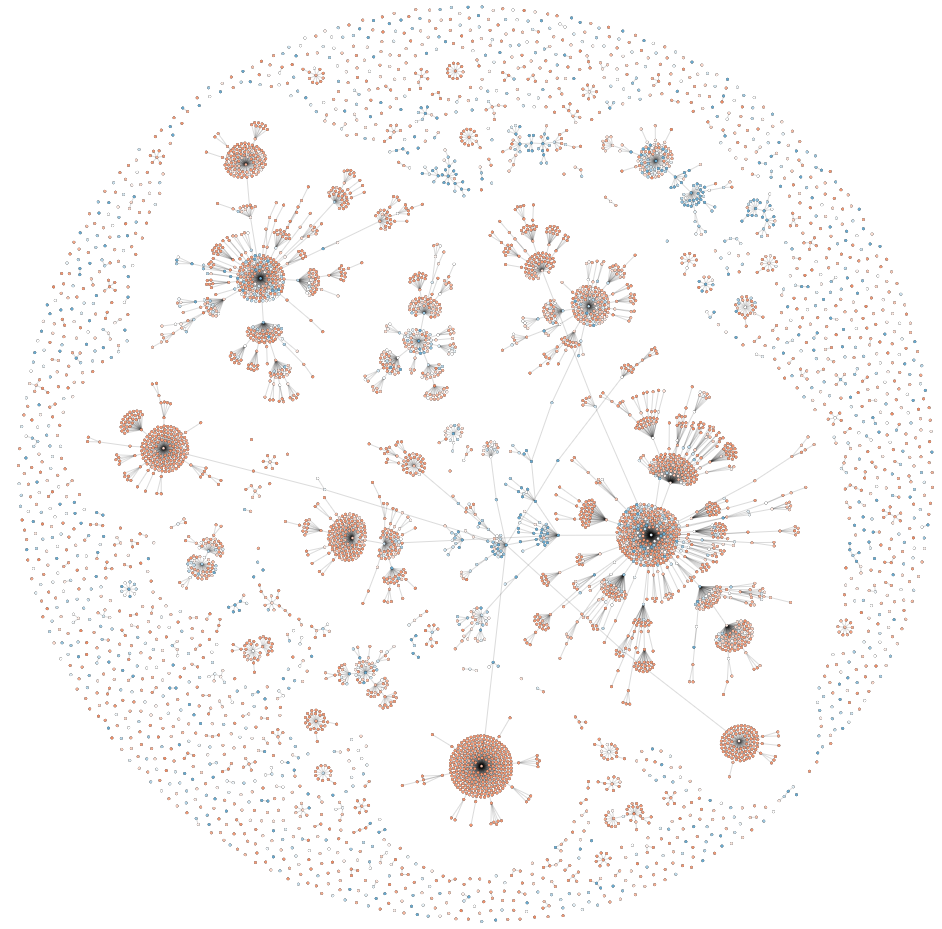
\includegraphics[width=0.5\linewidth]{figs/current/graph_d2}
\caption{
Node-link diagram showing how neighborhoods of data points are interconnected
with increasingly larger distances.
The edges of the directed graph always lead to points with a higher prediction score.
Especially of interest are label flips (ie., the prediction score increases by a wide
margin) or neighborhoods with consistent labels.
}
\label{figs:current_graph}
\end{figure}